\documentclass[11pt,a4paper]{report}
\usepackage[cm]{fullpage}
\usepackage{graphicx}
\usepackage{hyperref}
\usepackage{url}
\usepackage{glossaries}
\usepackage{listings}

\newacronym{ibm}{IBM}{Internation Business Machines}
\newacronym{rdf}{RDF}{Resource Description Framework}

\newcommand{\HRule}{\rule{\linewidth}{0.5mm}}

\begin{document}
\begin{titlepage}
\begin{center}
\HRule \\[0.4cm]
{ \huge \bfseries Sherlock}\\[0.0cm]
\HRule \\[0.0cm]
{ \large \emph{``Eliminate all other factors, and the one which remains must be the truth.''}}\\[2.0cm]
\begin{minipage}{0.4\textwidth}
\begin{flushleft} \large
\emph{Author:}\\
Alexander Brown\\
\ \\
\emph{Module:}\\
CS26210\\
\ \\
\emph{Assignment:}\\
A Chatbot in Prolog
\end{flushleft}
\end{minipage}
\begin{minipage}{0.4\textwidth}
\begin{flushright} \large
\end{flushright}
\end{minipage}
\vfill
{\large \today}
\end{center}
\end{titlepage}

\tableofcontents
\chapter{Design}
\section{Architecture}
The overall architecture of ``Sherlock'' is somewhat inspired by \gls{ibm} Watson. 
However due to the private nature of that code I can't completely base my 
design on Watson; a good choice due to the need for ``Sherlock'' to run 
without the aid of a mainframe.

Another design choice I'm keen to take is to use the \gls{rdf}, for which 
SWI-Prolog has an existing and supporting library.

The beauty of \gls{rdf} is that it has a predicate-based triplet structure, which
would make Input data for ``Sherlock'' very easy to both load and produce.

With time constraints it's unreasonable to expect ``Sherlock'' to learn over
time as many natural-language based systems tend to. As such AI conecepts
such as Neural Networks are also unreasonable.

With this in mind, what can be reasonably expected from ``Sherlock''?

\begin{enumerate}
\item Understand what the question is looking for.
\item Search a `database' of information for a given subject.
\item Respond with a sensible answer.
\end{enumerate}

Of the three, searching and responding are the simple modules; Natural 
Language processing being renound for being a complex field of AI.


\section{RDF Database}
\gls{rdf} are based on the idea of expressing simple statments with resources,
where each statement consists of a subject, a predicate and an object.

\begin{figure}[h!]
\textbf{http://www.example.org/index.html} has a \textbf{creator} whose value 
is \textbf{John Smith}

\centering
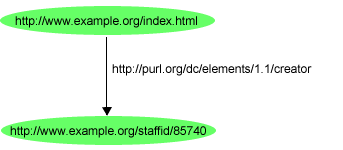
\includegraphics[scale=0.5]{img/fig2dec16.png}
\caption{A Simple RDF Statement\cite{website:w3_rdf_primer}}
\end{figure}

\gls{rdf} gets interesting when you consider joining objects. Nodes (subjects or 
objects) are connected using arcs (predicates). Nodes can be joined together
and chain down. Using the example given by the specification tadpole could be
represented by Figure~\ref{fig:tadpole}.

\begin{figure}[h!]
\centering
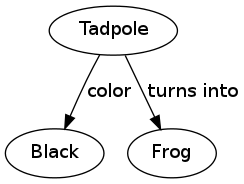
\includegraphics[scale=0.5]{img/tadpole.png}
\caption{An exaple of how the tadpole\label{fig:tadpole} example could be 
defined using the RDF graph structure.}
\end{figure}

So how does this help? Well Prolog works with predicates which are also an 
integral part of \gls{rdf}. So we can make logical connection in our database of
\gls{rdf}s.

The other neat part of \gls{rdf}s is that it takes away a number of prolems 
associated with the natural language processing as the predicates are a 
already in place and defined by the \gls{rdf}s (colour, turns into, etc.).

The final reason for going down an \gls{rdf} route is the extensibility of their
structure; potentially any data could be represented in the \gls{rdf} database
whilst being able to keep the base.


\section{Natual Language Processing}
With the use of \gls{rdf} databases to model data there's very little need to
do any actual natural language processing. That is to say, the question can 
be inferred from the words input and their existence in RDF data types, with
the inclusion of a database of synonyms (which can also be store in an RDF
structure). 

To solve this problem somewhat, answers from a synonym are reduced in weight
(the answer being returned as a confidence level, much like \gls{ibm} Watson
does).

To futher this approach the predicates of the found topics should be returned
and analysed to find any common themes and format it into the answer.

\chapter{The Nature of Understanding in the Context of Predicate Logic}

\section{What is Understanding?}
Understanding is a complex subject because it is a hard concept to grasp;
for a start knowledge does not imply understanding and vice versa. One can
have knowledge of all the parts of an engine and yet not understand how those
pieces fit together as a whole. On the flipside one can understand how engines
work but have no knowledge of the specific parts of an engine.

The Chinese Room is a thought experiment presented by John Searle and has very
close ties to computational understanding.

The overall principal of the Chinese Room is that a black box recieves messages 
in chinese, processes them using a set of rules and gives a response in chinese.
The operator of the box has no external contact (aside from the messages they 
recieve) and has no understanding of chinese.

The black box is evidently a metaphor for a computer (computers being very good
at performing large sets of instructions). The operator can appear to have a 
brilliant understanding of chinese depending on how encompassing the rules are.

However this brings about a interesting conundrum, as the human mind only works
using electrical signals - much as a computer does. So can the human mind truely
be replicated by a computer?

Given that we don't understand the full nature of the human mind yet, one cannot
say for sure. And the lines become even futher blurred when you add that a lot of
computers can `learn', quite similar to how humans do. Again I return to \gls{ibm} 
Watson which processes a huge amount of training data before it can produce any
useful answers. It can even learn from the mistakes it has made in the past so
that it can only improve.

So is this really understanding? Not entirely I would say. One thing all these 
knowledge-based systems cannot do at the moment is use their current knowledge
and invent their own knowledge. They may be able to uncover knowledge that has 
not been spotted before, even optimise existing solutions. But they currently
do not make the distrinctions between their many knowledge areas to improve
overall knowledge of both. Then, and only then, would I start considering 
reevaluating my position on whether computers can ever truely understand anything.

\section{``Sherlock'' and Understanding}
Sherlock's understanding comes from the input \gls{rdf} data, which is, at the end of
the day, produced by humans. Not computers.

I make no bones that Sherlock cannot understand the subject it represents, 
whatever that may be. However a part of Sherlock is about being able to 
understand the question it is being asked, understanding what is required for a response.

\chapter{Testing}
\lstinputlisting{testing.txt}

\chapter{Evaluation}
Due to a lack of time due to work commitments, ``Sherlock'' isn't as complete as it 
could be. For example there is currently a bug where it can be 200\% confident in a
given answer and not being able to respond with anything other than a confidence 
level when it should be able to return some sort of idea of what the question was
about.

Most of these issues would actually be easily fixed. The bug with 200\% confidence is
likely an issue which requires use of the cut (\verb+!+) operator. The not being able
to associate subject with the question (and answer) would be solved by being able to
store the predicates from the \gls{rdf} data.

\chapter{Code}
\section{ask.pl}
\lstinputlisting[language=prolog]{../src/ask.pl}
\newpage

\section{synonym.pl}
\lstinputlisting[language=prolog]{../src/synonym.pl}
\newpage

\section{rdf\_utils.pl}
\lstinputlisting[language=prolog]{../src/rdf_utils.pl}

\bibliographystyle{plain}
\bibliography{sherlock}

\end{document}
